\documentclass[10pt]{article}
\usepackage[final]{graphicx}
\usepackage{amsmath,mathrsfs}
\usepackage{amsfonts}
\usepackage[square, numbers, sort]{natbib}
\bibliographystyle{abbrvnat}
\newcounter{bibcount}
\bibliographystyle{unsrt}
\usepackage{bm}
\usepackage{ragged2e}
\usepackage[colorlinks]{hyperref}
\usepackage{multirow, booktabs}

\usepackage{url}

\topmargin-.5in
\textwidth6.6in
\textheight9in
\oddsidemargin0in

\def\ds{\displaystyle}
\def\d{\partial}

\usepackage{amsmath,amsfonts,amssymb,amsthm,epsfig,epstopdf,url,array}


\theoremstyle{plain}
\newtheorem{thm}{Theorem}[section]
\newtheorem{lem}[thm]{Lemma}
\newtheorem{prop}[thm]{Proposition}
\newtheorem*{cor}{Corollary}

\theoremstyle{definition}
\newtheorem{defn}{Definition}[section]
\newtheorem{conj}{Conjecture}[section]
\newtheorem{exmp}{Example}[section]

\theoremstyle{remark}
\newtheorem*{rem}{Remark}
\newtheorem*{note}{Note}


\begin{document}

\centerline{\large \bf Hybrid Splicing of Multi-Scale Downscaler Air Quality Surfaces}

\vspace{.1truein}

\def\thefootnote{\arabic{footnote}}
\begin{center}
  Elizabeth Herman\footnote{Department, University},
  Jeonghwa Lee\footnote{Department, University},
  Kartik Lovekar\footnote{Department, University},
  Dorcas Ofori-Boateng\footnote{Department of Mathematical Sciences, University of Texas at Dallas},
  Fatemeh Norouzi\footnote{Department, University},
  
  Benazir Rowe\footnote{Department of Mathematical Sciences, University of Nevada Las Vegas},
  Jianhui Sun\footnote{Department, University}
\end{center}

%\vspace{.1truein}

\begin{center}
Problem presenters: Elisabeth Mannshardt\footnote{Environmental Protection Agency}, Barron Henderson\footnote{Environmental Protection Agency}, and Brett Gantt\footnote{Environmental Protection Agency}

 
Faculty Mentor: Brian Reich\footnote{NCSU Statistics}
\end{center}

%%%%%%%%%%%%%%%%%%%%%%%%%%%%%%%%%%%%%%%%%%%%%%%%%%%%%%%%%%%%%%%%%%%%%%%%%%%%%%%%%%%%%%%%%%

\vspace{.3truein}
\centerline{\bf Abstract}

\justify
The current EPA air pollution prediction model uses downscaler model uses the same parameter $\phi$ that is the same for all continental United States. However if we could run downscaler model on smaller regions, the parameter $\phi$ of the downscaler model could be localized and therefore we expect it to yield more precise predictions.Regional and national downscaler air quality predictions differ significantly for regions where AQS density is low. We present a method to splice regional downscaler air quality surfaces for regions with both low and high discrepancies.  The method provides visual smoothing of the 2 overlapping surfaces and can be extended to handle higher dimensional overlap.  We use the data from the downscaler models ran separately on 9 NOAA climatic regions of the continental US with some overlaps. Since tuning parameter is now different for each region there are significant discrepancies in the areas where the density of AQS stations is low. Such regions are Northwest, North Rockies, West and Southwest regions. 
We focus on providing the smoothed estimates for the overlap areas based on predictions from 2 downscaler models. We base our smoothing parameter based on the latitudinal distance to the edge of both of the downscaler regions. In case if point lies close to the boundary of the region, the predictions from this region should be given less weight. 
We provide an approach to generate smoothed estimates for overlap regions that blend in the discrepancies between 2 predictions based on the distance from the point to the boundary.
%%%%%%%%%%%%%%%%%%%%%%%%%%%%%%%%%%%%%%%%%%%%%%%%%%%%%%%%%%%%%%%%%%%%%%%%%%%%%%%%%%%%%%%%%%

\section{Introduction}

\justify
In 2016, the US EPA estimated that approximately 123 million people lived in 
counties where air quality concentrations were above the primary EPA's NAAQS \cite{EPAAir}.  Additionally, the World Health Organization (in 2018) also reported an estimate of about 7 million premature deaths caused by ambient air pollution for the same timeline \cite{WhoAir}.  Research, over the years, has established linkage between exposure to Particulate Matter (PM) and health-related risks such as respiratory diseases \cite{schwartz1996air, braga2001lag, dominici2006fine}.  $PM_{2.5}$ describes fine inhalable particles, with 2.5 micrometers and smaller diameters.  As a regulatory body, the EPA is able to control pollutant concentration levels with information coming from two sources - Monitoring sites and Output from complex numerical models that produce concentration surfaces over large spatial regions.\\
\vspace{-1.5em}
\justify
From these sources of information, the following data products are obtained:
\begin{itemize}
	\vspace{-0.5em}
	\item Air Quality System (AQS) measurements: Measurements of air pollutant concentrations from a monitoring network throughout the United States.
	\vspace{-0.5em}
	\item Community Multi-scale Air Quality (CMAQ) model: Simulations that combine current knowledge in atmospheric science and air quality modeling and multi-processor computing techniques to produce pollutant estimates.
	\vspace{-0.5em}
	\item Downscaler Model (DS): Model which fuses CMAQ output with air pollution readings using a spatially weighted model that regresses a monitoring data on a CMAQ derived regressor.
	\vspace{-0.5em}
	\item Inter-agency Monitoring of Protected Visual Environments (IMPROVE): Multi-agency monitor network to collect visibility related data.
\end{itemize}

\justify
In recent decades, the attempt to fuse the two sources of information has allowed the EPA to provide downscaler Air Quality surfaces on a national spatial scale \cite{berrocal2010bivariate, berrocal2010spatio}.  However, predictions on regional scales produce an unsmoothed national surface.  This is illustrated in Figure~\ref{fig:Regional overlapping}\\~
\begin{figure}[!ht]
	\centering
	\vspace{-5em}
	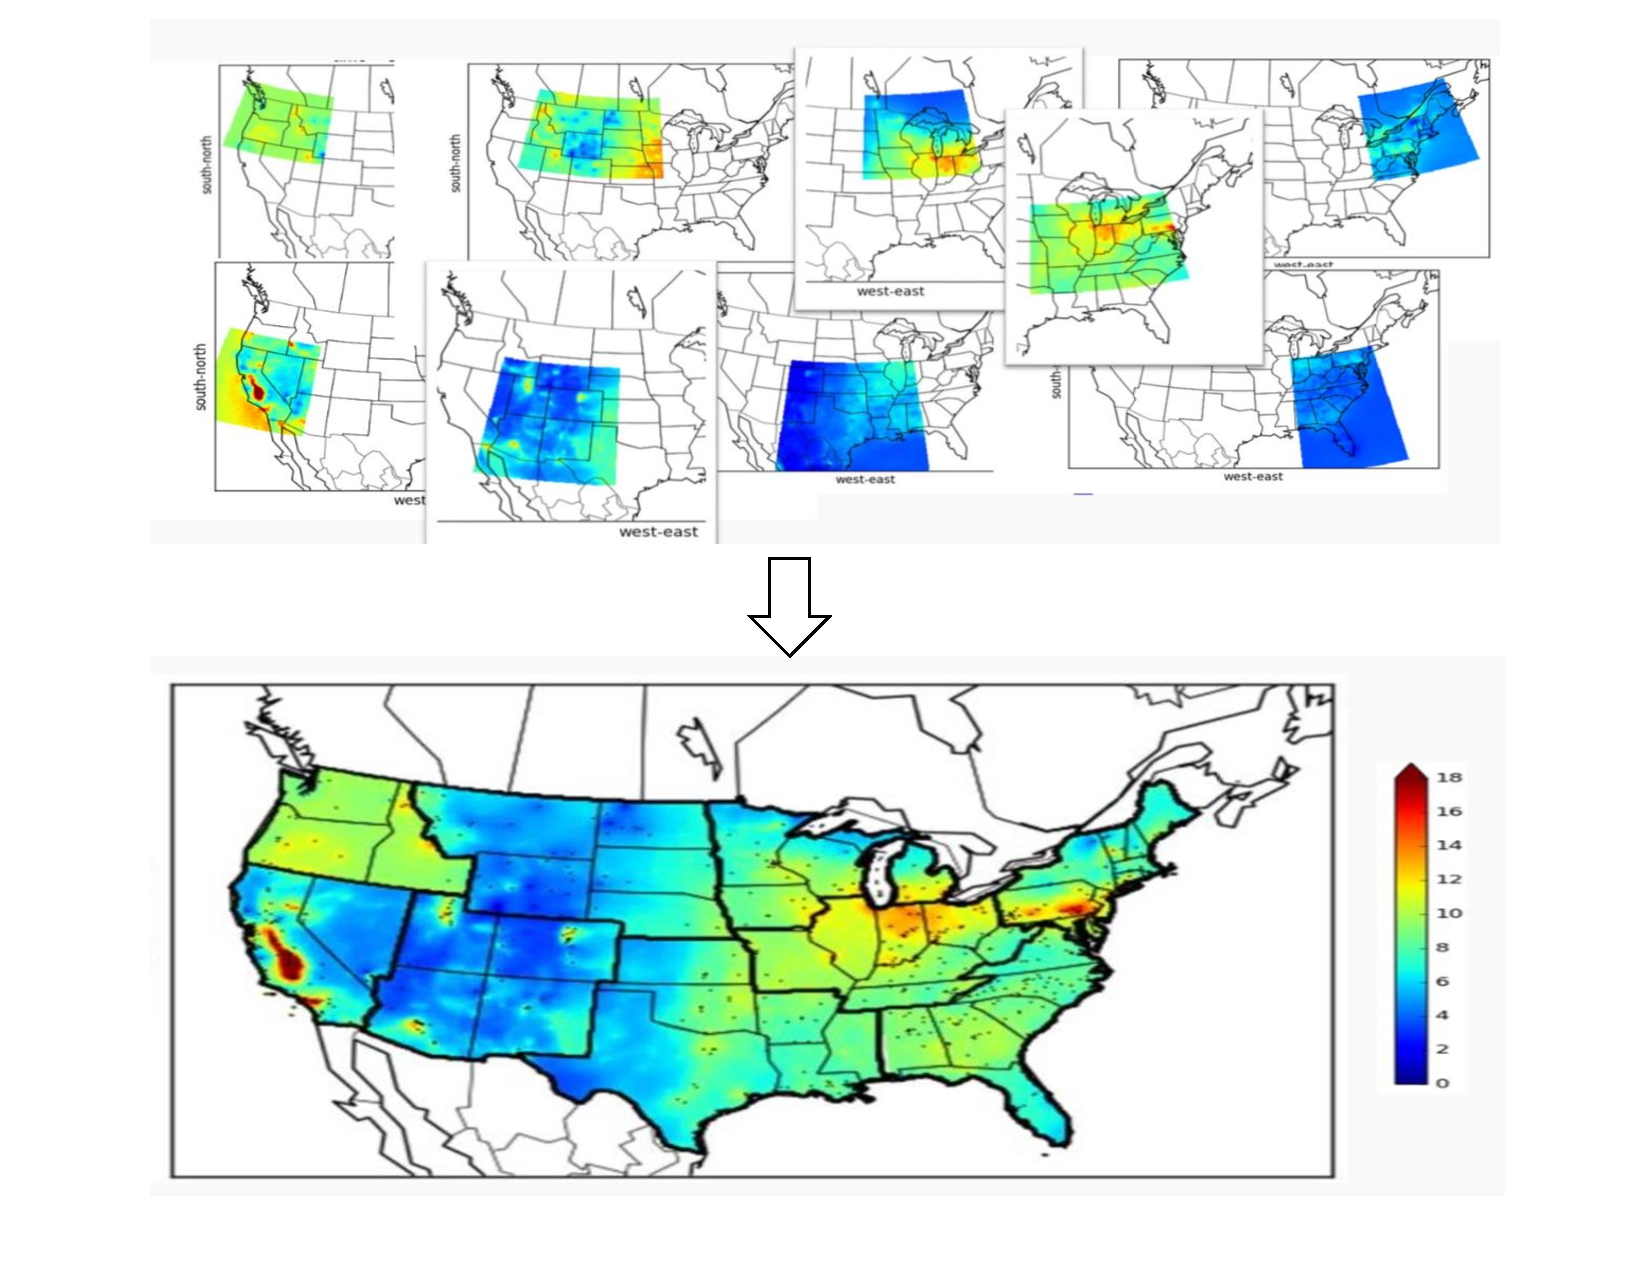
\includegraphics[width= 16cm, scale = 1, height = 11cm]{Image_1}
	\caption{Name of Figure}
	\label{fig:Regional overlapping}
\end{figure}

\justify
With this study, we intend to build a methodological splicing framework/algorithm for regional estimates along regional boundaries to create smooth national surface.

%%%%%%%%%%%%%%%%%%%%%%%%%%%%%%%%%%%%%%%%%%%%%%%%%%%%%%%%%%%%%%%%%%%%%%%%%%%%%%%%%%%%%%%%%%

\section{Data}
\justify
The data comes from three sources, AQS sites, IMPROVE sites, and evaluations of the Downscaler model.  The data we looked at was data collected in Quarter 1.  That is, the data we are considering was collected in January, February, and March.  The methodology we will develop below can be extended to any quarter of the year.  Below, we will discuss how the data source is collected, why the data source is beneficial, and the limitations we have using the data.  We will begin with the data collected at the AQS sites. 
\justify
The AQS data was collected at AQS sites.  These sites have AQS machines on the ground to collect concentrations of pollutants (specifically $PM_{2.5}$, the pollutant we are interested in).  We will henceforth refer to this data as AQS data  or the ``ground truth''.  While we do have actual readings of the concentration of $PM_{2.5}$, this data is usually only collected near large cities.  The reason for this is that there is legislation that requires cities of certain populations to purchase a machine and then use it to collect readings of pollution in the air.  Additionally, the data is not collected every day.  For instance, there are locations that collect data every six (6) days.  As a result, it is difficult to get a consistent amount of reliable data from these machines.  Note also that we are not considering the effects of noise in data collection (\textit{i.e.} no measurement noise in our data collection).
\justify
Our second source of data comes from IMPROVE sites.  These sites are again measuring the concentration of the pollutant $PM_{2.5}$ in the air.  Unlike the AQS sites, these sites are located in areas in which there is not a high concentration of the pollutant.  For instance, the IMPROVE sites can be located in a National Park or other rural areas.
\justify
Our last piece of data we will be using is from a model called Downscaler (DS).  This model works on a grid, the continental United States divided into 12 km by 12 km pieces.  It essentially uses a ``fancy'' linear regression to incorporate the data gathered from the AQS sites and another source of information that indicates the type of environment the grid block is located at.  The output of Downscaler is a mean and standard error for each grid point.  Because the Downscaler is an evaluation of a model, we can choose the area in which we run the model. This is the source of our problem.  Normally, the Downscaler is 
ran on a national scale.  That is, it incorporates all of the data from the AQS sites located in the continental United States.  The potential problem with this, is that if the location we are trying to extrapolate is in the NW, the model considers the readings of the AQS machines in the SE.  The hypothesis is that while there is some correlation between the regions in close proximity to each other, overall, the concentrations of $PM_{2.5}$ on one side of the country do not have an effect on the readings on the other side of the country.  The proposed solution is to run the Downscaler on a regional scale with overlapping areas in-between the regions.  Consequently, a specific grid point only includes information that is "relevant" to the region that it is in.  We include an overlap region because it is assumed that the grid points on the edge of the boundary will be impacted by the near-by grid points in the adjacent region.  Two questions arise from this proposed solution: what regions should be used? and how do we deal with the overlapping region?

\justify
We will address the first question by splitting the continental United States by the NOAA climate zones.  This means that we will have nine regions that we are running the Downscaler on.  The nine regions are Northwest (NW), Northern Rockies (NR), Upper Midwest (UM), Ohio Valley (OV), Northeast (NE), Southeast (SE), South (S), Southwest (SW), and West (W).  Recall that we are considering these zones plus some overlap into the adjacent regions. Figure~\ref{fig:US} shows the continental US broken up into the NOAA Climate Zones.

\begin{figure}
	\centering
	\vspace{-2em}
	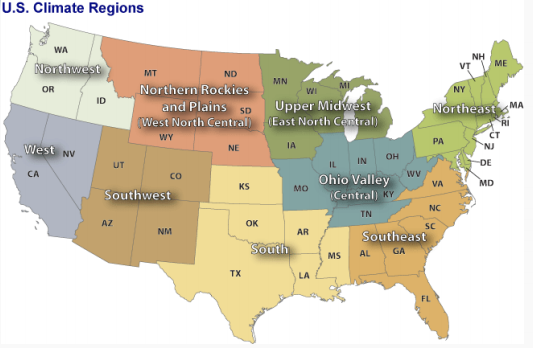
\includegraphics[width= 10cm, scale = 1, height = 7cm]{ContUS}
	\caption{NOAA Climate Zones.}
	\begin{flushleft}
	Source: \href{https://www.epa.gov/sites/production/files/2016-05/us-climate-regions_0.gif}{NOAA National Climatic Data Center} 
	\end{flushleft}
	\label{fig:US}
\end{figure}


\justify
The second question is the reason for which we are writing this paper.  Because we are running the Downscaler for each region plus some overlap, the overlap area will have two (or more) DS values for which the Downscaler model provides an evaluation at each gridpoint.  This paper seeks to provide a methodology for this overlap region.  An example of the overlap region is provided in Figure~\ref{fig:overlap}.  Notice that the boxes represented by the dashed lines are the NOAA Climate Zones, i.e. they are a collection of states defined by NOAA in which the states have similar climates.  The two regions that we ran Downscaler on are represented by the solid lines.  By running the Downscaler twice, in the overlap region (which includes the NOAA Climate Zone boundary) we have an evaluation of Downscaler at each grid point.  As a result, we need to find a way to combine the two evaluations into one that makes sense for the grid point.

\begin{figure}
	\centering
	\vspace{-1em}
	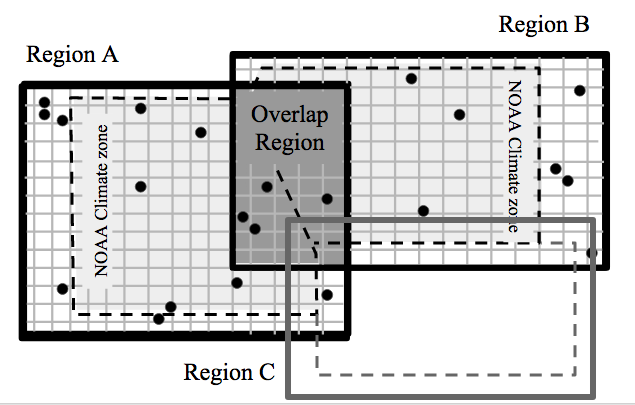
\includegraphics[width=0.7\linewidth]{overlap}
	\caption{Name}
	\label{fig:overlap}
\end{figure}

%%%%%%%%%%%%%%%%%%%%%%%%%%%%%%%%%%%%%%%%%%%%%%%%%%%%%%%%%%%%%%%%%%%%%%%%%%%%%%%%%%%%%%%%%%

\section{Methodology}
In this section we describe diverse approaches considered to attain the objective of smooth splicing. We consider the following approaches.\\
%Method 1:
Suppose that, for the site $s$, the distribution of DS from region $i$ is a Normal distribution with mean $\hat{\mu_{i}(s)}$ and standard deviation $\hat{\sigma_{i}(s)}$, (for i = 1,2).
\justify
In order to splice the information coming from both regions in the overlap region, we propose the Model averaging below (equation number). The probability density function (pdf) at $s$ is characterized by a weighted average of pdfs from $\bm{R}_{1}$ and $\bm{R}_{2}$. 

\begin{equation}\tag{1.1}\label{1.1}
f = w_{1}(s)f_{1,s} + w_{2}(s)f_{2,s}
\end{equation}
\justify
where $f_{i}$ is Normal density function with $\mu = \hat{\mu_{i}(s)}, \sigma = \hat{\sigma_{i}(s)}$, and $w_{i}$ is the region assigned weight.  The weight is set as a function of a distance between $s$ and the outer boundary in the overlap. 


\justify
This quantification is because the closer the site is to the outer line of a region, the lesser it will be affected by the information from the region.  In other words, $w_{i}(s)$ is proportional to the distance of the site $s$ to the outer boundary of region $i$ in the overlap, and the farther the point is toward the inner area of region $i$ the lesser it will be influenced by the adjacent region.  
Figure XXX provides a summary illustration of the above discussion.

(picture-horizontal distance)

\justify
If the intersection of two regions lies up and down, then the distances are obtained by vertical distances of $s$ to the boundaries as shown in the figure below.

(picture-vertical distance)

\justify
To adjust for the effect of the distance on the weight, a parameter $\phi$ is introduced.  Therefore the weight $w_{i}(s) $ is defined as:

\begin{equation}\tag{1.2}\label{1.2}
w_{i}(s) = e^{-\phi d(s,i)}
\end{equation}

\justify
where $d(s,i) $ is the  distance of point $s$ to outer boundary of region $i$ (for $i =  1,2$). For a  larger $\phi$ , the distance measure $d(s,i)$ has a  larger influence on the weight, giving the distribution from each region a stronger effect on near area.  
On the other hand, the smaller the $\phi$ the more the two distributions are blended in the overlap.  In the case where $\phi$ is zero , the weights become evenly distributed among the densities (\textit{i.e.} $w_{i}(s)=.5$ for $i=1,2$).  For $\phi=\infty$  the probability density function $f$ at $s$ simply becomes either $f_{1,s}$ or $f_{2,s}$ 
depending on which boundary is closer to $s$, thus the weight has no effect on the averaging.
(picture-weight function with different phi) 

\justify
Armed with the above assumptions and deductions, we derive the following likelihood function for  AQS $y_j$  at $s_j \in R_{1} \cap R_{2}  , j = 1,.., n.$

\begin{align*}    
\mathcal{L} (y_1,..,y_n; \phi) &= \prod_{j=1}^{n} f(y_j) = \prod_{j=1}^{n}  w_{1}(s)f_{1,s}(y_j) + w_{2}(s)f_{2,s}(y_j)              \\
&         = \prod_{j=1}^{n} e^{-\phi d(s_j,1)}f_{1,s_j}(y_j) +  e^{-\phi d(s_j,2)}f_{2,s_j}(y_j)
\end{align*}



%%%%%%%%%%%%%%%%%%%%%%%%%%%%%%%%%%%%%%%%%%%%%%%%%%%%%%%%%%%%%%%%%%%%%%%%%%%%%%%%%%%%%%%%%%

Using maximum likelihood method, $\hat{\phi}$ is obtained, and the new predicted mean at the site $s$ in the overlap becomes weighted means :
\begin{align}
\hat{\mu(s)} &=\int y \hat{f(y)} dy= \int \hat{w_{1}(s)}f_{1,s}(y)+\hat{w_{2}(s)}f_{2,s}(y) \\ & = 
\int   y \exp(-\hat{\phi} d(s,1))f_{1,s}(y)+y \exp(-\hat{\phi} d(s,2))f_{2,s}(y) dy \\ &=   \exp(-\hat{\phi} d(s,1))\hat{\mu_{1}(s)}+ \exp(-\hat{\phi} d(s,2)) \hat{\mu_{2}(s)} \\
&=\hat{w_{1}(s)}\hat{\mu_{1}(s)}+ \hat{w_{2}(s)}\hat{\mu_{2}(s)} \end{align}   where $\hat{w_{i}(s)}=\exp(-\hat{\phi} d(s,i)), i=1,2.$\\
\par (M2) Method 2:
\\ Instead of mixing density functions, here we mix two random variables. Assume that we have two independent normal variables at site $s$ in the overlap, each from DS region $i, i=1,2.$ In other words, for a site $s$  the information from DS region $i$  is assumed to be represented by $X_{i}(s) \sim N( {\hat \mu_{i}(s)}, {\hat \sigma_{i}(s)}   ),    i=1,2.$
Our new combined information at site $s$ is then expressed as follows:
\[ X= w_{1}(s)X_{1}(s)+w_{2}(s)X_{2}(s)\] where the weight $w_{i}(s)$ is defined as before,
$w_{i}(s)=\exp(-\phi d(s,i)).$
With the assumption that $X_{1}(s)$ and $X_{2}(s)$ are independent normal variables, X becomes normal variable 
with mean $ \mu_{\phi}=  w_{1}(s){\hat\mu_{1}(s)}+w_{2}(s){\hat\mu_{2}(s)}$ and variance $ {\sigma_{\phi}}^2={w_{1}(s)}^2{\hat\sigma_{1}(s)}^2+{w_{2}(s)}^2{\hat \sigma_{2}(s)}^2$. 
Therefore the following likelihood function is as follows:
\[  \mathcal{L} (y_1,...,y_n;\phi)= \prod_{j=1}^{n}f(y_j;\phi)  \] where $f(y;\phi)$ is normal density function with mean $\mu_{\phi}$ and variance
${\sigma_{\phi}}^2.$

Using maximum likelihood method, MLE of $\phi$, $\hat{\phi}$, is obtained yielding new predicted mean at the site $s$ in the overlap as
${\hat\mu(s)} ={\hat w_{1}(s)}{\hat \mu_{1}(s)}+ {\hat w_{2}(s)}{\hat \mu_{2}(s)},   $ where ${\hat w_{i}(s)}=\exp(-\hat{\phi} d(s,i)).$\\
\par (M3) Method 3:\\ 
Here the whole procedure is the same as M2 except that the parameter $\phi$ is  now  a linear function of horizontal distance of site $s$ in the overlap to the
vertical center line in the overlap area.

(pic of distance to explain it)

The reason we set the parameter as a function of this distance is because  the degree of influence of distance on weight could be different when the site is in the middle than it lies close to outer lines.
More specifically, we have the following function for $ \phi$: 
\[ \phi(d(s,c))= b_0+b_1 d(s,c)   \] where $d(s,c)$ is the horizontal distance of $s$ to the  vertical center line, i.e.,  $d(s,c)=|s_{lon}-c_{lon}|$ where
$s_{lon}, c_{lon}$ are longitude of point $s$ and center line $c$ respectively.

(possibly pic??for this)

By using this function for $\phi$, we can make the surface smoother in the middle while the edge of the overlap remain closer to the inner area than we use constant $\phi$ as in M2.


%%%%%%%%%%%%%%%%%%%%%%%%%%%%%%%%%%%%%%%%%%%%%%%%%%%%%%%%%%%%%%%%%%%%%%%%%%%%%%%%%%%%%%%%%

\subsection{smooth surfaces from three methods}
Since the regional DS shows that the most disconnected region is the area between NW and NR, we restric ourselves to these regions, 
applying the three methods in the previous section on the overlap of NW and NR.
The following is the results from each method:


\begin{table}[!ht]
	\centering
	\caption{MLE}
	\label{table:name of table for referncing}
	\begin{tabular}{ l l l l l l l} 
		\toprule
		& &  \multicolumn{5}{c}{Method (M)} \\ \cmidrule(l){3-7} 
		Parameter & &  M1      & &  M2       & &   M3 \\
		\toprule
		$\phi$    & &   1.450  & &  0.222    & &   -    \\
		$b_{0}$   & &   -      & &  -        & &   0.157 \\
		$b_{1}$   & &   -      & &  -        & &   0.029 \\
		\bottomrule
	\end{tabular}
\end{table}


The above table shows MLE of parameter in each method.
For M1 and M2, we have one parameter $\phi$ and for M3 we have $b_0 ,$ $b_1$ in weight function. The MLE of $\phi$ is 1.450, 0.222 for M1 and M2 respectively meaning that M2 smooth the data in the overlap more than M1 since it has larger $\hat{\phi}$. For M3, $\hat{b_0}=0.157  ,\hat{b_1}=0.029.$



\begin{figure}[!ht]
	\centering
	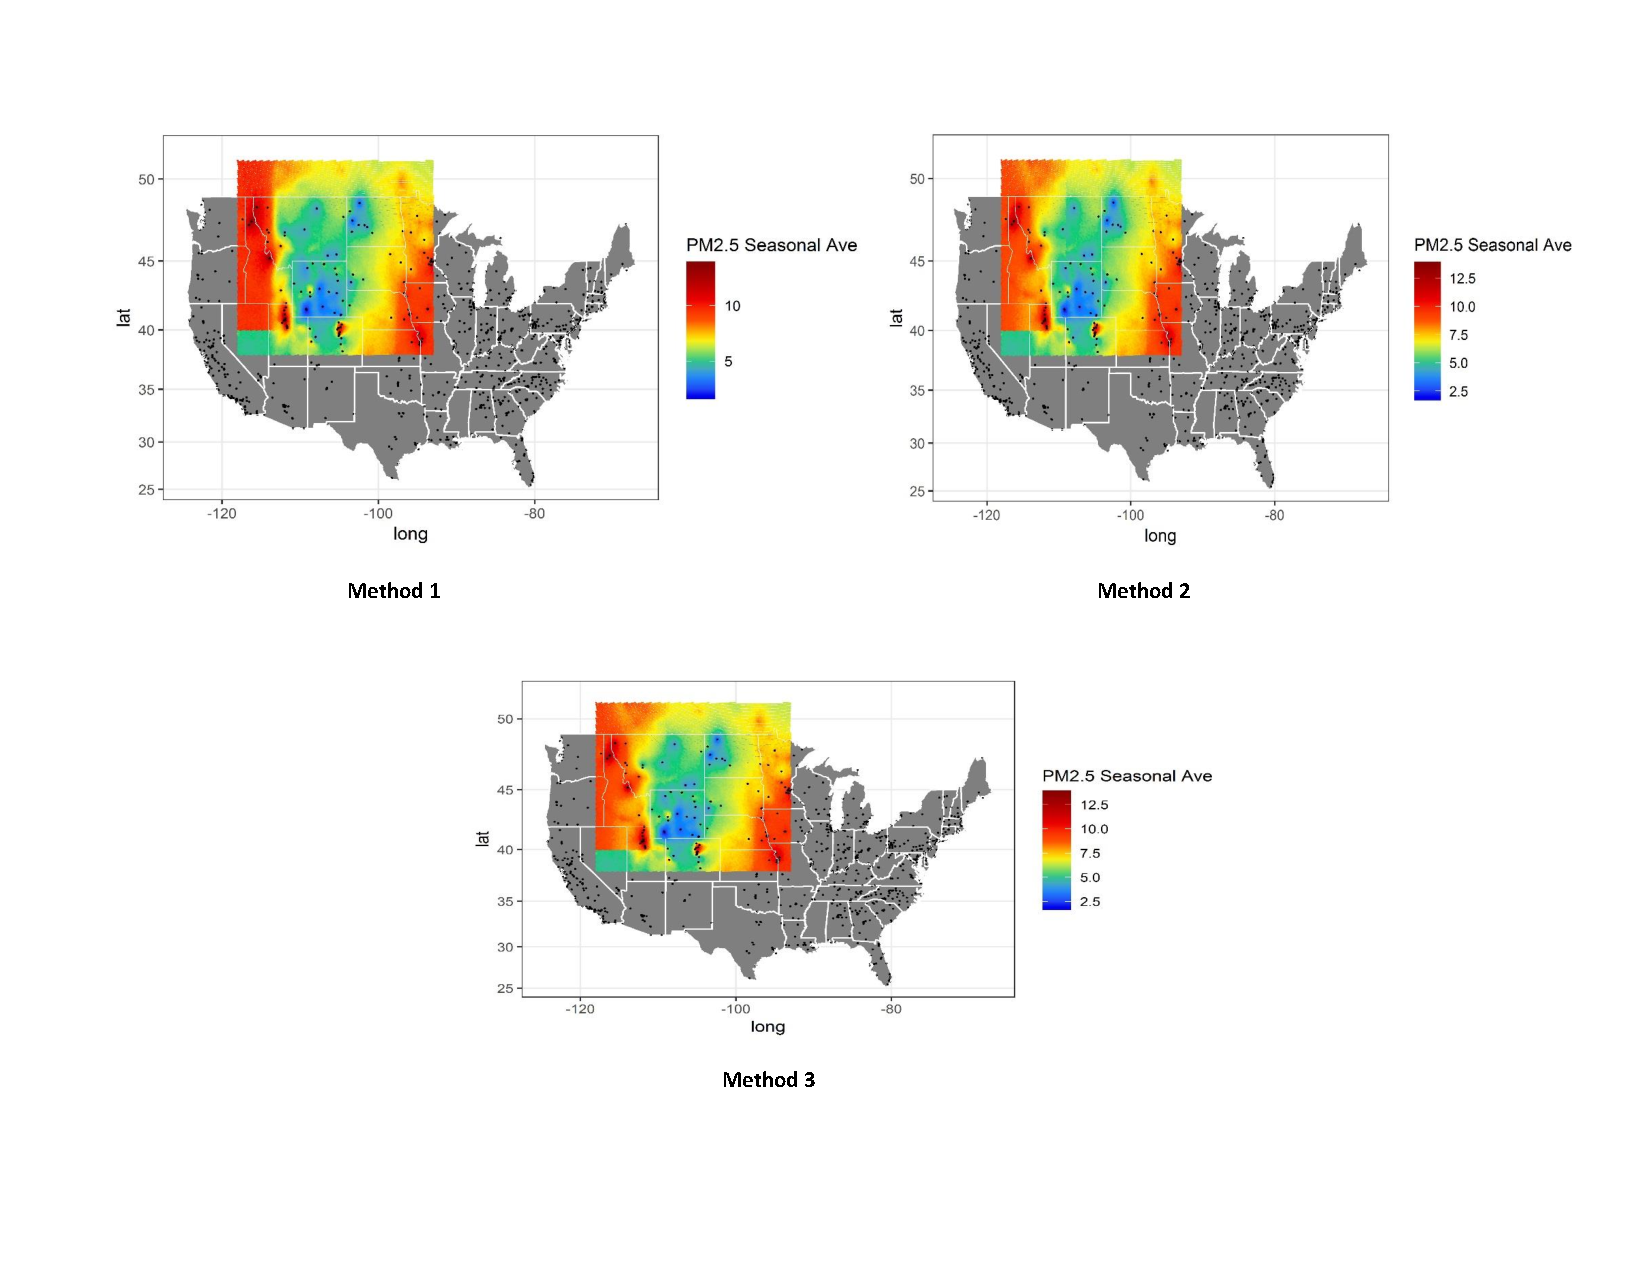
\includegraphics[width = 18cm, scale = 1, height = 10cm]{All_Methods}
	\vspace{-5em}
	\caption{ (a) M1 applied on the intersection of NR and NW (b) M2 applied on the intersection of NR and NW  (c) M3 applied on the intersection of NR and NW 
		\vspace{-1em}
		\label{fig: Applying M1, M2, M3 on the intersection of NR and NW}}
\end{figure}


\justify
It is clear from the picture 1 and picture 2 that M2 shows smoother surface than M1 as we can see the sharp red edge in the middle in picture 1.
This result looks puzzling in the first place, makes one wondering why M2 makes smoother surface. This can be explained  when pdfs are drawn for the two methods.
(graph of pdfs from two methods )
\justify
The black and red graph above are drawn with two normal densities, $N(0,1), N(3,1)$ with weight $.3, .7 $ from M1 and M2 respectively. The blue graph is drawn with the same densities but with weights $.1,.9$ respectively with M1. 
The means of the black and red density are the same, $.21.$
Density function from M2 is normal density, symmetric, and has a peak at the mean. 
Density function from M1 is skewed to the left which has smaller weight, and has peak at 3.  The peak in M1 is 3 when the second weight is larger than .5, highest when the weight is .5, and  getting lowered making more skewed distribution as 
the weight is decreased. This can be seen by comparing the blue and black graph. 
It is that property that makes MLE of $\phi$ in M1 larger than that of M2, making the values in the overlap stay closer to the mean from closer area,
thus produce less smooth surface.
\justify
Comparing the picture 2 and 3, it is seen that the method 3 is better at smoothing near the outer boundary of NW region,
since we see the disconnection on the outer boundary  of NW on picture 2 and it is blurred in picture 3. This result is 
expected as we make $\phi$ as a linear function of distance from the center line. 


\begin{rem}
	There are many other ways to splice two regions making smooth surface. If one uses different form of $\phi$, and/or different distance
	measure, different smooth surface might be obtained. In this study we only use either longitude of sites or latitude of sites  for splicing two region to measure the distance but one can also use both latitude and longitude achieving smoothness in both direction-horizontally and vertically.
	Also  $\phi$ can be  quadratic form of distance making more dynamic smooth surface.
	Here we want to mention that there could be a case where different smooth surfaces produced by different methods are all very smooth and at the same time they all fit the data well. Then splicing surfaces could be subjective matter in that case , and it is because of the lack of data in particular region. 
	Nontheless our method is not too complicated and useful tool when two different information on the same region needs to be combined.
	
\end{rem}

\subsection{comparing methods using cross validation}



\subsection{comparing methods using MSE}

\justify
MSE(mean square error)
In our data, it turned out that the M fits the data best as it has the smallest MSE. 
PMSE(predicted mean squared error)
M has the smallest PMSE among three models in our case. We make comment that it doesn't mean that Mis always fits the data best nor
Mis superior than the other methods. 




%%%%%%%%%%%%%%%%%%%%%%%%%%%%%%%%%%%%%%%%%%%%%%%%%%%%%%%%%%%%%%%%%%%%%%%%%%%%%%%%%%%%%%%%%%

\section{Computational Experiments}
Give enough details so that readers can duplicate your experiments.

\begin{itemize}
	\item Describe the precise purpose of the experiments, and what they 
	are supposed to show.
	
	\item Describe and justify your test data, and any assumptions you made to 
	simplify the problem.
	
	\item Describe the software you used, and the 
	parameter values you selected.
	
	\item 
	For every figure, describe the meaning and units of the coordinate axes, 
	and what is being plotted.
	
	\item Describe the conclusions you can draw from your experiments
\end{itemize}

%%%%%%%%%%%%%%%%%%%%%%%%%%%%%%%%%%%%%%%%%%%%%%%%%%%%%%%%%%%%%%%%%%%%%%%%%%%%%%%%%%%%%%%%%%

\section{Summary and Future Work}
\begin{itemize}
	\item Briefly summarize your contributions, and their possible
	impact on the field (but don't just repeat the abstract or introduction).
	\item Identify the limitations of your approach.
	\item Suggest improvements for future work.
	\item Outline open problems.
\end{itemize}



\bibliography{mybib3} 
%\bibliographystyle{plainnat}
\bibliographystyle{ieeetr}


%%%%%%%%%%%%%%%%%%%%%%%%%%%%%%%%%%%%%%%%%%%%%%%%%%%%%%%%%%%%%%%%%%%%%%%%%%%%%%%%%%%%%%%%%%



\end{document}